\section{编写教程}
本章节介绍如何使用本模板编写电子电路与系统基础的学习资料。本章节不会出现在正式分发的文件中，仅供同学学习使用。
\subsection{前期准备}
\subsubsection{安装\LaTeX{}编译环境}
在编写之前，请确保您已经安装了\LaTeX{}编译环境。具体请安装TeX Live， 同时安装VsCode并在其上安装LaTeX Workshop插件。安装后，需要将默认编译引擎更换为XeLatex。方法为：
\begin{enumerate}
  \item 打开VsCode，点击插件，点击Latex Workshop插件的设置按钮，选择“扩展设置”。
    \item 找到“{\tt Latex-workshop > Latex > Recipe: Default}" 选项并将其修改为“{\tt latexmk (xelatex)}”。
\end{enumerate}
\subsubsection{安装git}
我们将基于git进行协作。请首先在\url{https://github.com}注册一个账号，并将它发给我（江玮陶），我将将你拉进本项目的协作组。\footnote{如果由于网络问题你无法访问github，请参考\url{https://register.wallesspku.org}的解决方案。}然后请在你的电脑上安装git，具体请参考\url{https://docs.eesast.com/docs/tools/git}。对于mac用户，只需要在终端运行指令
\begin{lstlisting}[language=bash]
brew install git
\end{lstlisting}
即可安装git。安装git后，请按照如下方法配置ssh key以便于后续操作：
\begin{enumerate}
  \item 在终端中运行如下指令，生成ssh key：
\begin{lstlisting}[language=bash]
ssh-keygen -t rsa -b 4096 -C "your_email@example.com"
\end{lstlisting}
  其中请将\texttt{your\_email@example.com}替换为您在GitHub上注册的邮箱地址。
    \item 在github网站上，进入Settings页面，选择SSH and GPG keys选项卡，点击New SSH key按钮。
    \item 在Title栏中输入一个名称（例如“我的电脑”），然后将刚才生成的ssh key内容粘贴到Key栏中。ssh key内容可以通过运行如下指令获得：（其中路径可能因系统和配置不同而异，请根据实际情况修改）
\begin{lstlisting}[language=bash]
cat ~/.ssh/id_rsa.pub
\end{lstlisting}
    \item 点击Add SSH key按钮完成添加。
\end{enumerate}

\subsubsection{协作工作流}
在完成上述步骤后，您就可以开始协作编写文档了。

\noindent\emph{首次克隆项目}

在您的电脑上打开终端，运行如下指令克隆项目到本地：
\begin{lstlisting}[language=bash]
git clone git@github.com:CBDT-JWT/CAD-cookbook.git

\end{lstlisting}
\noindent\emph{日常更新与提交}

在日常编写过程中，请按照如下步骤进行更新与提交：
\begin{enumerate}
  \item 在开始编写之前，先运行如下指令拉取最新的代码：
\begin{lstlisting}[language=bash]
git pull origin master
\end{lstlisting}
    \item 在完成编写后，运行如下指令将修改添加到暂存区：
\begin{lstlisting}[language=bash]
git add .
\end{lstlisting}
    \item 运行如下指令提交修改：
\begin{lstlisting}[language=bash]
git commit -m "你的提交信息"
\end{lstlisting}
    \item 运行如下指令将修改推送到远程仓库：
\begin{lstlisting}[language=bash]
git push origin master
\end{lstlisting}
\end{enumerate}

\noindent\emph{编译文档}

如果你使用vscode中的latex workshop插件，可以使用快捷键{\tt ctrl+s} (mac 为{\tt cmd+s})直接编译文档。

\subsection{\LaTeX{}基础}
\begin{center}
    {\Huge \textbf{TBD}}
\end{center}

\subsubsection{段落格式}
每个chapter文件应当独立作为一个{\tt section}, 即在段落开头使用
\begin{lstlisting}[language=TeX]
\section{章节标题}
\end{lstlisting}
来定义章节标题。章节内可以使用{\tt subsection}和{\tt subsubsection}来定义子章节。每个自然段前后应当空一行，段和图片之间也要空一行。

\subsubsection{数学公式}
数学公式可以使用美元符号{\tt \$}来包裹行内公式，例如：{\tt \$E=mc\^{}2\$}会渲染为$E=mc^2$。行间公式可以使用{\tt \$\$ ... \$\$}来包裹，例如：
\begin{lstlisting}[language=TeX]
$$
\begin{cases}
\nabla \cdot \mathbf{E} = \frac {\rho} {\varepsilon_0} \\
\nabla \cdot \mathbf{B} = 0 \\
\nabla \times \mathbf{E} = - \frac {\partial \mathbf{B}} {\partial t} \\
\nabla \times \mathbf{B} = \mu_0 \mathbf{J} + \mu_0 \varepsilon_0 \frac {\partial \mathbf{E}} {\partial t}
\end{cases}
$$
\end{lstlisting}

会渲染为：
$$
\begin{cases}
\nabla \cdot \mathbf{E} = \frac {\rho} {\varepsilon_0} \\
\nabla \cdot \mathbf{B} = 0 \\ 
\nabla \times \mathbf{E} = - \frac {\partial \mathbf{B}} {\partial t} \\
\nabla \times \mathbf{B} = \mu_0 \mathbf{J} + \mu_0 \varepsilon_0 \frac {\partial \mathbf{E}} {\partial t}
\end{cases}
$$

常用的数学符号可以参考\url{https://zhuanlan.zhihu.com/p/472919794}。

\subsubsection{表格}
表格可以使用{\tt table}环境来创建，例如：
\begin{lstlisting}[language=TeX]
\begin{table}[htbp]
    \centering
    \caption{示例表格} %表格标题
    \label{tab:example} %表格标签，方便引用
    \begin{tabular}{|l|c|r|} %这里l表示左对齐，c表示居中，r表示右对齐
    \toprule %表格顶部横线
    Header 1 & Header 2 & Header 3 \\
    \midrule %表格中部横线
    Cell 1 & Cell 2 & Cell 3 \\
    Cell 4 & Cell 5 & Cell 6 \\
    \bottomrule %表格底部横线
    \end{tabular}
\end{table}
\end{lstlisting}
会渲染为：

\begin{table}[htbp]
    \centering
    \caption{示例表格}
    \label{tab:example}
\begin{tabular}{l|c r} %这里l表示左对齐，c表示居中，r表示右对齐

\toprule %表格顶部横线
Header 1 & Header 2 & Header 3 \\
\midrule %表格中部横线
Cell 1 & Cell 2 & Cell 3 \\
Cell 4 & Cell 5 & Cell 6 \\
\bottomrule %表格底部横线
\end{tabular}
\end{table}

可以使用{\tt \textbackslash ref\{tab:example\}}的方式在正文中引用表格，例如“如表\ref{tab:example}所示”。在实际使用中，可以使用\url{https://www.tablesgenerator.com}方便地制作表格。

\subsubsection{插入图片}
图片可以使用{\tt figure}环境来插入，例如：
\begin{lstlisting}[language=TeX]
\begin{figure}[htbp]
    \centering
    
\includegraphics[width=0.5\textwidth]{chapters/figure/example.png} %插入图片，width参数控制图片宽度，chapters/figure/example.png为图片路径
    \caption{示例图片} %图片标题
    \label{fig:example} %图片标签，方便引用
\end{figure}
\end{lstlisting}

会渲染为图\ref{fig:example1}和\ref{fig:example2}所示。

\begin{figure}[htbp]
    \centering
    
\includegraphics[width=0.5\textwidth]{chapters/figure/example.png}
    \caption{示例图片}
    \label{fig:example}
\end{figure}
可以使用{\tt \textbackslash ref\{fig:example\}}的方式在正文中引用图片，例如“如图\ref{fig:example}所示”。请将图片文件放置在项目的{\tt figure}文件夹中。如果想要并列多张图片，可以使用minipage环境，例如：
\begin{lstlisting}[language=TeX]
\begin{figure}[htbp]
    \centering
    \begin{minipage}{0.45\textwidth}% 设置图片宽度为文本宽度的45%
        \centering
        
\includegraphics[width=.9\textwidth]{chapters/figure/example1.jpeg}
        \caption{示例图片1}
        \label{fig:example1}
    \end{minipage}
    \hfill
    \begin{minipage}{0.45\textwidth}
        \centering
        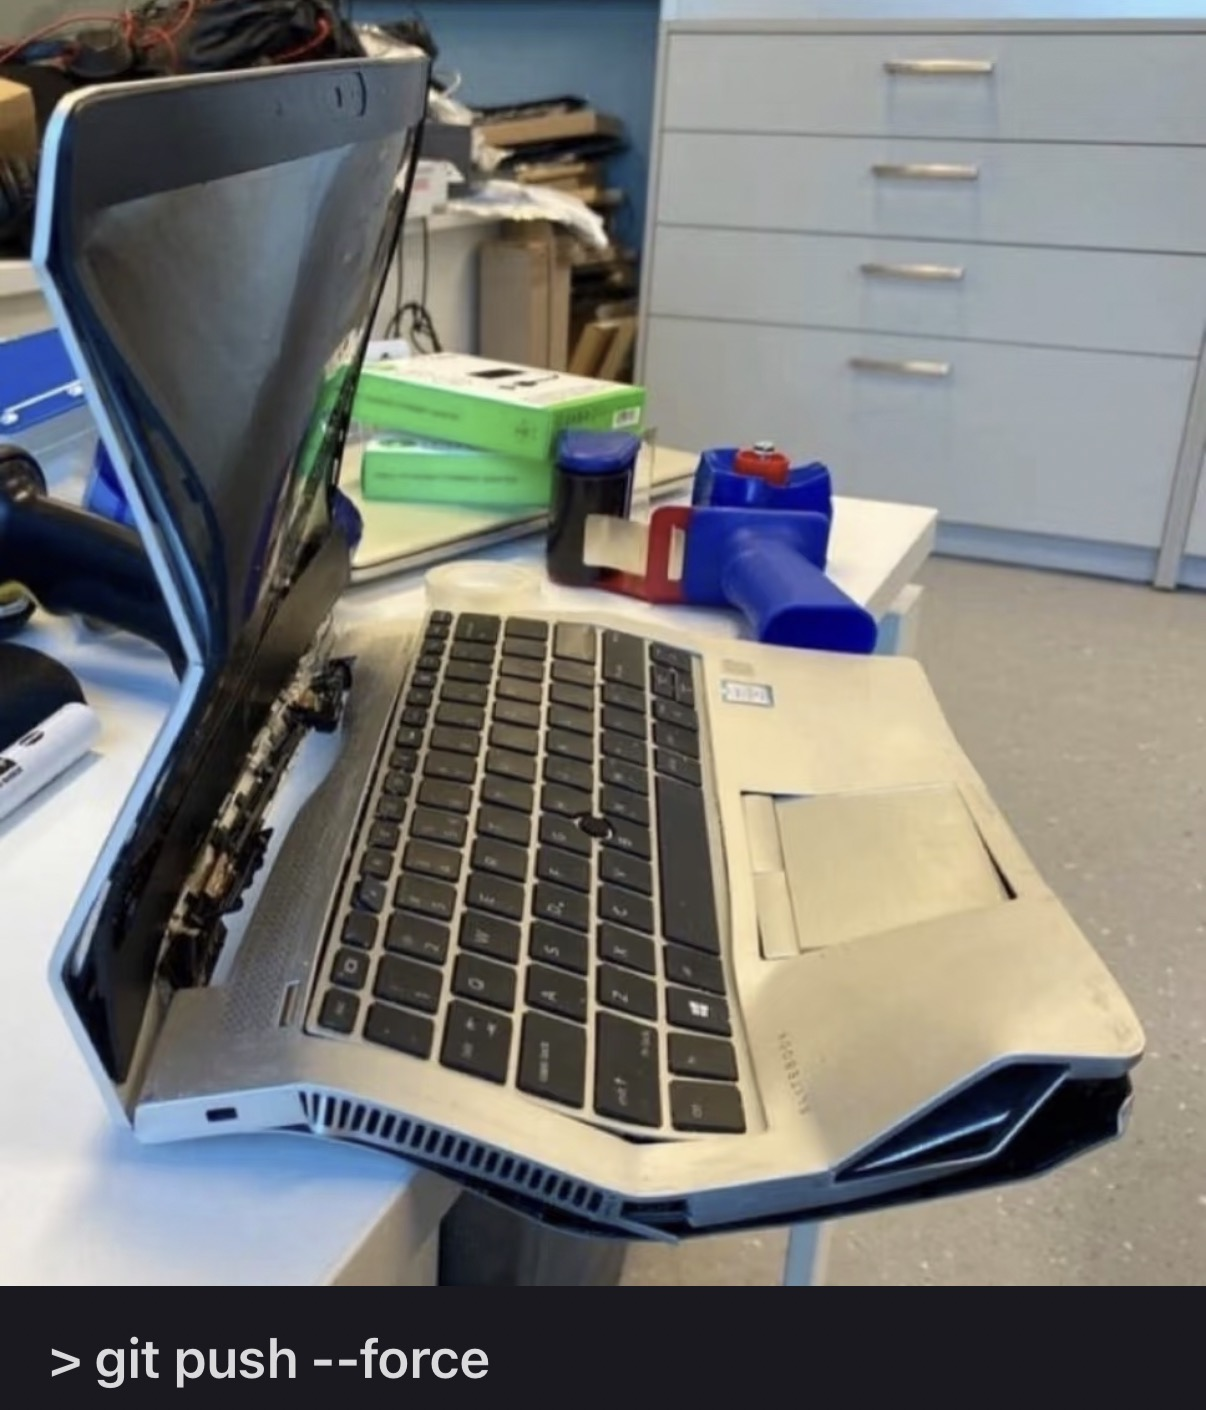
\includegraphics[width=.9\textwidth]{chapters/figure/example2.jpeg}
        \caption{示例图片2}
        \label{fig:example2}
    \end{minipage}
\end{figure}
\end{lstlisting}
会渲染为：

\begin{figure}[htbp]
    \centering
    \begin{minipage}{0.45\textwidth}
        \centering
        
\includegraphics[width=\textwidth]{chapters/figure/example1.jpeg}
        \caption{示例图片1}
        \label{fig:example1}
    \end{minipage}
    \hfill
    \begin{minipage}{0.45\textwidth}
        \centering
        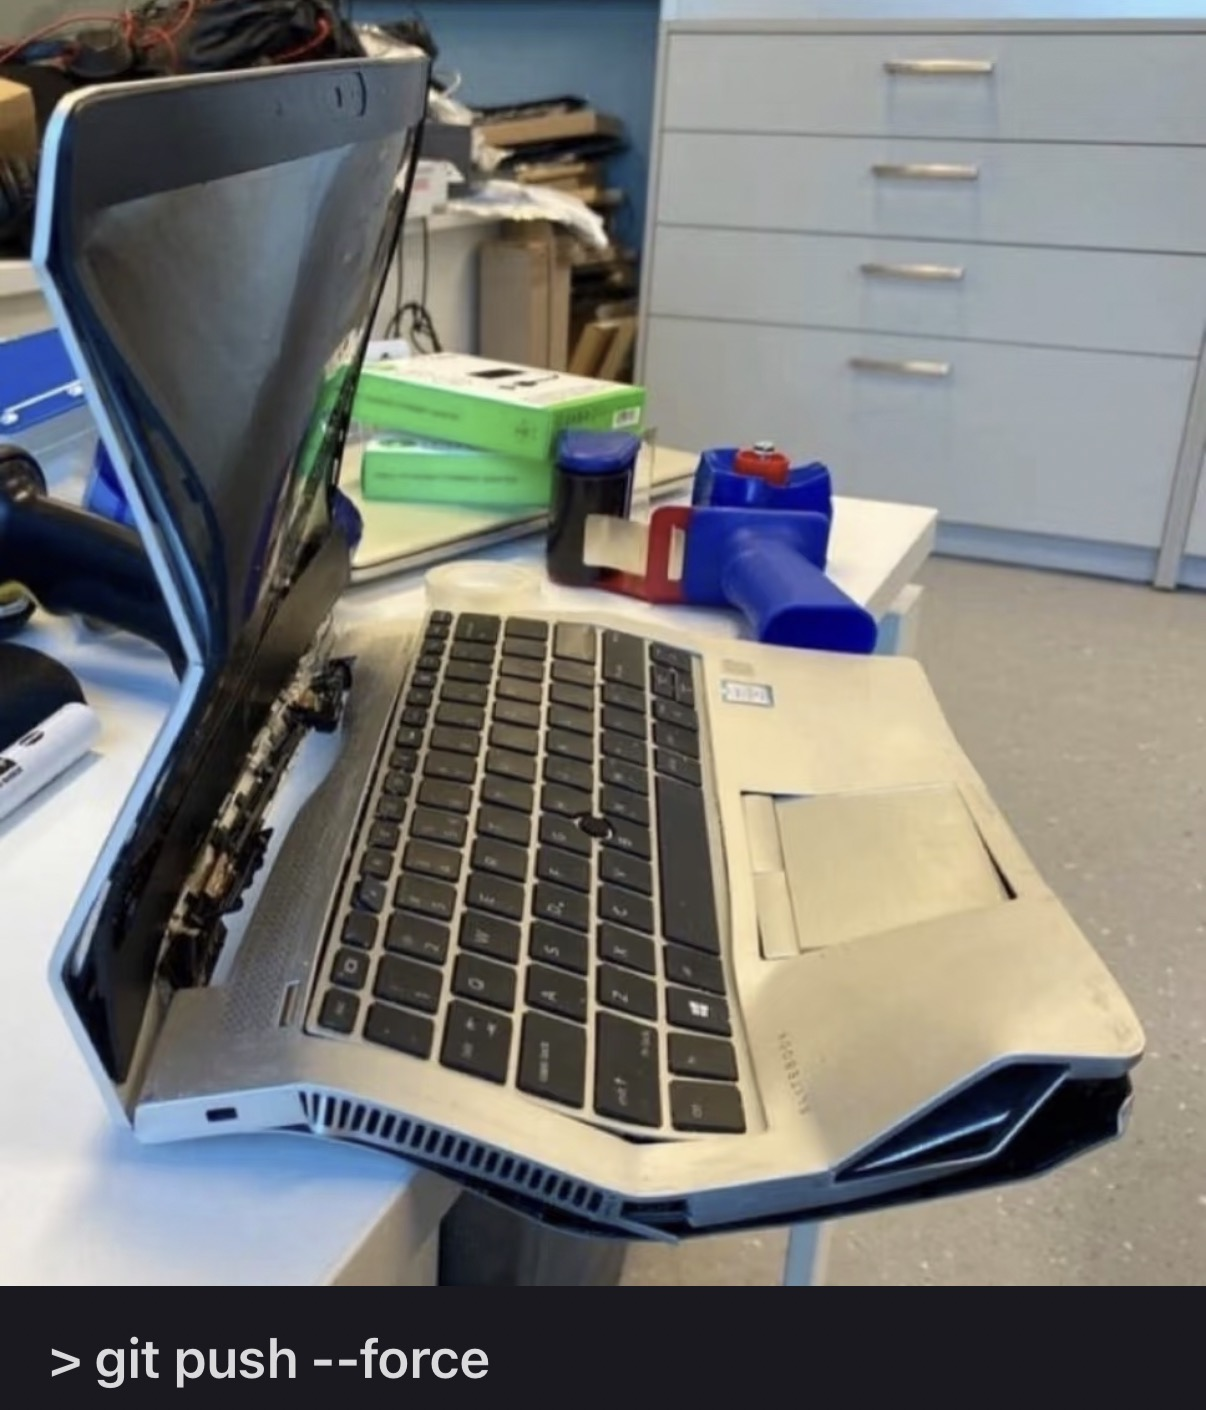
\includegraphics[width=\textwidth]{chapters/figure/example2.jpeg}
        \caption{示例图片2}
        \label{fig:example2}
    \end{minipage}
\end{figure}

\noindent\emph{电路图绘制}\quad 为了统一，我们采用circuitikz宏包绘制电路图。具体使用方法请参考\url{https://www.jiangwt.org/docs-html/documents/circuitikz/}。下面是一个简单的例子：
\begin{lstlisting}[language=TeX]
\begin{figure}[htbp]
    \centering
    \resizebox{0.6\textwidth}{!}{%
    \begin{circuitikz}
    \tikzstyle{every node}=[font=\LARGE]
    \draw (3.25,10) to[european resistor,l={ \LARGE $R_s$}] (5.5,10);
    \draw (9.25,9) to[Tnpn, transistors/scale=1.19] (9.25,11);
    \draw (5.5,10) to[C] (7.5,10);
    \node at (7.5,10) [circ] {};
    \draw (7.5,10) to[european resistor,l={ \LARGE $R_{B1}$}] (7.5,12.5);
    \draw (7.5,7.5) to[european resistor,l={ \LARGE $R_{B2}$}] (7.5,10);
    \draw (7.5,10) to[short] (8.25,10);

    \draw (7.5,7.5) to (7.5,7.25) node[ground]{};
    \draw (9.25,9) to[european resistor,l={ \LARGE $R_E$}] (9.25,7);
    \draw (9.25,7) to (9.25,6.75) node[ground]{};
    \draw (9.25,11) to[european resistor,l={ \LARGE $R_C$}] (9.25,13.25);
    \draw (8.75,13.25) to[short] (9.75,13.25);
    \draw (7,12.5) to[short] (8,12.5);
    \draw (3.25,10) to[american voltage source] (3.25,8.5);
    \draw (3.25,8.5) to (3.25,8.25) node[ground]{};
    \draw (9.25,10.75) to[C] (11.25,10.75);
    \draw (11.25,10.75) to[european resistor,l={ \LARGE $R_L$}] (11.25,8);
    \draw (11.25,10.75) to[short, -o] (12,10.75) ;

    \draw (11.25,8.75) to (11.25,8.5) node[ground]{};
    \end{circuitikz}
    }%
    \caption{样例电路}
    \label{fig: example-circuit}
\end{figure}
\end{lstlisting}


\begin{figure}[h!]
    \centering
    \resizebox{0.6\textwidth}{!}{%
    \begin{circuitikz}
    \tikzstyle{every node}=[font=\LARGE]
    \draw (3.25,10) to[european resistor,l={ \LARGE $R_s$}] (5.5,10);
    \draw (9.25,9) to[Tnpn, transistors/scale=1.19] (9.25,11);
    \draw (5.5,10) to[C] (7.5,10);
    \node at (7.5,10) [circ] {};
    \draw (7.5,10) to[european resistor,l={ \LARGE $R_{B1}$}] (7.5,12.5);
    \draw (7.5,7.5) to[european resistor,l={ \LARGE $R_{B2}$}] (7.5,10);
    \draw (7.5,10) to[short] (8.25,10);

    \draw (7.5,7.5) to (7.5,7.25) node[ground]{};
    \draw (9.25,9) to[european resistor,l={ \LARGE $R_E$}] (9.25,7);
    \draw (9.25,7) to (9.25,6.75) node[ground]{};
    \draw (9.25,11) to[european resistor,l={ \LARGE $R_C$}] (9.25,13.25);
    \draw (8.75,13.25) to[short] (9.75,13.25);
    \draw (7,12.5) to[short] (8,12.5);
    \draw (3.25,10) to[american voltage source] (3.25,8.5);
    \draw (3.25,8.5) to (3.25,8.25) node[ground]{};
    \draw (9.25,10.75) to[C] (11.25,10.75);
    \draw (11.25,10.75) to[european resistor,l={ \LARGE $R_L$}] (11.25,8);
    \draw (11.25,10.75) to[short, -o] (12,10.75) ;

    \draw (11.25,8.75) to (11.25,8.5) node[ground]{};
    \end{circuitikz}
    }%
    \caption{样例电路}
    \label{fig: example-circuit}
\end{figure}

会渲染为图\ref{fig: example-circuit}所示。实际使用中，circuitikz直接写代码绘制电路图可能比较麻烦，建议使用\url{https://tikzmaker.com/editor}在线编辑器绘制电路图，然后将生成的代码复制到文档中。